%% USE one of these:
%% * the first when using pdflatex, which directly typesets your document in the
%%   chosen pdf/a format and you want to publish your thesis online,

%% * the second when you want to print your thesis to bind it, or
%% * the third when producing a ps file and a pdf/a from it.
%%
\documentclass[english, 12pt, a4paper, sci, utf8, a-1b, online]{aaltothesis}

\usepackage{graphicx}
%% Math fonts, symbols, and formatting
\usepackage{amsfonts,amssymb,amsbsy,amsmath,amsthm,enumitem,mathtools,braket,tikz}
\usepackage[capitalize]{cleveref}
\usepackage[parfill]{parskip}
\usepackage{hyphenat}
% \usepackage[style=ieee]{biblatex}
% \addbibresource{zotero.bib}

\hyphenpenalty=10000
\tolerance=1000

%% added by advisor
\usepackage{xcolor}
\newtheorem{theorem}{Theorem}
\newtheorem{lemma}[theorem]{Lemma}
\newtheorem{corollary}[theorem]{Corollary}
\theoremstyle{definition}
\newtheorem{definition}{Definition}
\theoremstyle{remark}
\newtheorem{remark}{Remark}

% advisor
\newcommand{\fda}[1]{{\color{red} \textbf{Francesco}: #1}}

% own notes
\newcommand{\TODO}{{\color{red} \textbf{TODO!} }}
\newcommand{\note}[1]{{\color{purple} \emph{#1} }}

% math commands
\newcommand{\rsquared}{{ \ensuremath{\mathbb{R}^2 }}}
% \newcommand{\nngrid}{{ n_{1}n_{2} }}
\newcommand{\nngrid}{{ \ensuremath{n_{1}n_{2}} }}

% a configuration C is a mapping ...
\newcommand{\conf}[1]{\ensuremath{\mathcal{C}_{#1}}}
% inverse of a configuration
\newcommand{\iconf}[2]{\conf{#1}^{-1}(#2)}
% normal configuration with (#2)
\newcommand{\nconf}[2]{\conf{#1}(#2)}
% text and with spacing 
\newcommand{\tand}{MD\text{ and }}

\newcommand{\sopt}{S_\text{opt}}

\newcommand{\mono}[1]{\texttt{#1}}

\newcommand{\NP}{\text{NP}}
\newcommand{\pclass}{\text{P}}
\newcommand{\true}{\texttt{true}}
\newcommand{\false}{\texttt{false}}

\newcommand{\colvec}[2]{\ensuremath{\begin{pmatrix}
			#1 \\
			#2
\end{pmatrix}}}

\newcommand{\diagdegs}{\ensuremath{45^\circ\ }}

\newcommand{\schedules}{\ensuremath{\mathcal{S}}}

% set using parentheses
\newcommand{\parens}[1]{(\, #1 \,)}

\newcommand{\coord}[2]{(#1, \; #2)}

% euclidean norm
\DeclarePairedDelimiter{\euclnorm}{\lVert}{\rVert_2}
% manhattan norm
\DeclarePairedDelimiter{\manhattan}{\lVert}{\rVert_1}
% infty norm
\DeclarePairedDelimiter{\linfty}{\lVert}{\rVert_\infty}
% absolute value
\DeclarePairedDelimiter{\abs}{\lvert}{\rvert}



%% THESIS INFO
\degreeprogram{Computer Science}

\major{Computer Science}

\code{SCI3028.kand}

\univdegree{BSc}

\thesisauthor{Peik Etzell}

\thesistitle{Coordinated multi-robot motion planning: An overview}

\place{Espoo}

\date{\today}

\supervisor{Professor Eero Hyvönen}

\advisor{Postdoctoral researcher \\Francesco d'Amore}

\uselogo{aaltoRed}{''}

%% THE ENGLISH ABSTRACT:
%% Thesis keywords:
\keywords{}

%% The abstract text. This text is included in the metadata of the pdf file as well
%% as the abstract page.
\thesisabstract{
TODO
}

%% Copyright text. Copyright of a work is with the creator/author of the work
%% regardless of whether the copyright mark is explicitly in the work or not.
%% You may, if you wish, publish your work under a Creative Commons license (see
%% creativecommons.org), in which case the license text must be visible in the
%% work. Write here the copyright text you want. It is written into the metadata
%% of the pdf file as well.
%% Syntax:
%% \copyrigthtext{metadata text}{text visible on the page}

\copyrighttext{Copyright \noexpand\copyright\ \number\year\ \ThesisAuthor}
{Copyright \copyright{} \number\year{} \ThesisAuthor}


\begin{document}

%% Create the coverpage
\makecoverpage


%% Typeset the copyright text.
%% If you wish, you may leave out the copyright text from the human-readable
%% page of the pdf file. This may seem like a attractive idea for the printed
%% document especially if "Copyright (c) yyyy Eddie Engineer" is the only text
%% on the page. However, the recommendation is to print this copyright text.
\makecopyrightpage


%% ENGLISH ABSTRACT
%% All the details (name, title, etc.) on the abstract page appear as specified
%% above.
\begin{abstractpage}[english]
    \abstracttext{}
\end{abstractpage}

%% Force new page so that the Swedish abstract starts from a new page
\newpage

%% SWEDISH ABSTRACT.
\thesistitle{}
\supervisor{Professor Eero Hyvönen} 
\advisor{Postdoctoral researcher Francesco d'Amore}
\degreeprogram{Datateknik}
\major{Datateknik}
\keywords{}
\begin{abstractpage}[swedish]
TODO
\end{abstractpage}


% %% PREFACE
% %% This section is optional.
% \mysection{Preface}

% \vspace{5cm}
% Espoo, \today

% \vspace{5mm}
% {\hfill Peik Etzell \hspace{1cm}}

\newpage


%% TABLE OF CONTENTS
\thesistableofcontents

\clearpage

% INTRODUCTION
\section{Introduction}
\subsection{Background}

Robotic motion planning is a field of research in theoretical computer science which has been deeply studied. It focuses on designing and studying algorithms for making robots get from one point to another safely (without colliding) and efficiently (minimizing some properly defined cost function) \cite{mit/chosetPrinciplesRobotMotion2005}.

Robots are modeled in a vast number of ways, which differ in terms of shapes, sizes and kinematics: some warehouse robots can be modeled to move in two dimensions only, while flying drones can be seen as moving in three dimensions.

Robotic arms that move an end-effector are often modeled in six dimensions: three spatial ones and three for orientation. These robotic arms often have so-called kinematic redundancy, meaning they have more degrees of freedom than strictly necessary \cite{robo/ChiaveriniOM16}. Kinematic redundancy increases the fault-tolerance and dexterity of the robot, and makes it possible to re-adjust while hold the same end-effector pose, but it also increases the complexity in motion planning as poses can have different alternative joint configurations \cite{robo/ChiaveriniOM16}. Kinematic redundancy enables the arm to re-adjust while holding the same end-effector pose, which helps dexterity and fault-tolerance, but also increases complexity in planning, as poses can have different alternative joint configurations \cite{robo/ChiaveriniOM16}.

There are many different environments in which robots exist. Assembly line robots have a fairly static environment, well defined start and end positions, and a clear and safe path between them. Robotic vacuum cleaners on the other hand need to map their environment and make decisions dynamically, as furniture, people and pets can change places from time to time. Some robots need to work together; multi-robot systems can be found in warehouses \cite{robo/ParkerRS16}, where parallel motion is highly desirable, but past research has focused mostly on algorithms moving robots one-by-one \cite{siamcomp/DemaineFKMS19}.

\subsection{Parallel robots}

The field of coordinated motion planning for parallel robotics has seen a lot of research in recent years, with algorithms tackling different problems in the field. 

The many real world scenarios to be studied led to the formulation of different problems. The goal is to move the robots from their starting positions to their target positions without colliding with other robots. Without accounting for collisions, finding a solution would of course be trivial, as robots could move straight to their targets. There are two different general types of motion problems: finding a collision-free schedule transforming a workspace from a starting configuration to a target configuration is called a \emph{motion planning problem}, while determining if such a schedule exists is called the \emph{mover's problem} \cite{siamcomp/HopcroftW86}. 

After executing a valid schedule, all robots will have moved from their starting positions to their target positions, and all target positions are occupied by a robot.

Some variations to this motion problem exist: in its \emph{labeled} formulation, robots are unique, and are assigned specific target locations to move to. This problem formulation is the most studied \cite{fun/BrockenHKLS21}. In its \emph{unlabeled} formulation, robots are instead indistinguishable from each other, and targets can be occupied by any robot. In 2014, \cite{ijrr/SoloveyH14} introduced a generalization of labeled and unlabeled problems: in a \emph{(k-)colored} problem, the robots are partitioned into $k$ colors or groups, and each have to move to a target location with the same coloring. \emph{Labeled} and \emph{unlabeled} are then extremes of the \emph{colored} problem formulation: $k=1$ gives an unlabeled problem, as all robots are of the same color, while $k=n$ gives all robots their own unique color. 

% The problem has multiple variations: \refactor{we}{something else}
% in the unlabeled formulation of the problem, we do not care which robot gets to which target position, only that all target positions get occupied. 
% \TODO in the labeled formulation, robots and target positions have labels...
% In case we want to move specific robots to specific targets, we have a labeled problem, where robots and target positions each have labels, such that target positions contain a robot with the same label at the end. 
% Note that such labels can be unique or not, and some works distinguish between these cases: for example, \cite{demaineCoordinatedMotionPlanning2019} considers \emph{unlabeled, colored} and \emph{labeled} as variations on the problem, where \emph{labeled} means unique labels, and \emph{colored} is a generalization of the unlabeled and labeled variants: multiple robots (and targets) can have the same color, and the targets are only to be matched up with robots of the same color. \TODO explicit extreme
% Thus both the unlabeled and labeled formulations can be modeled as specific cases of the colored one.

Real robots are physically three-dimensional objects, but they are mostly restricted to two dimensions in multi-robot applications. There are some works exploring higher dimensions: \cite{arobots/TurpinMMK14}, but current works are quite focused on the two-dimensional setting. Reasons for this might be ease of visualization and thus understanding, simpler algorithms, real world applicability or something else.

The problem can also be modeled both in the continuous or discrete space. In a discrete model, the workspace is modeled as a grid, which can then be handled using graph theory, with grid cells being nodes that the robots occupy and move through.

In a continuous model, the robots can in theory be modeled as close to reality as wanted, but the increased complexity seems to not be worth it. Most current research in motion planning consider only simple shapes, and real warehouse robots also seem to reflect this in their shapes: many are shaped close to circles or squares. Unit radius disks (see \cite{siamcomp/DemaineFKMS19}, \cite{compgeom/BanyassadyBBBFH22}) or unit squares (see \cite{jea/YangV22}) make collision checking a lot simpler: a single distance metric on two robots' centers determines if they are in collision or not. Most continuous space research also study uniform sizes and shapes of robots, but for example \cite{fun/BrockenHKLS21} investigates motion planning of non-uniformly-sized discs.

% Finding the minimum makespan solution to a discrete grid case of the coordinated motion planning problem is found to be NP-hard by \cite{siamcomp/DemaineFKMS19}. \cite{siamcomp/DemaineFKMS19} also conjectures that the continuous formulation of the problem would be at least as hard, but leaves it for future work.
% NP-hardness implies approximation algorithms are justified \cite{siamcomp/DemaineFKMS19}, so research is focused on better approximations and faster computation. 

There is also a distinction between centralized and distributed computing in motion planning. Robots are inherently physically distributed, and a lot of research considers multi-robot systems as a problem of distributed computing. Most research in specifically robotic motion planning uses centralized planning though, where a single entity computes all moves for all robots. Distributed computing considers similar but distinct problems, like \emph{rendezvous} and \emph{exploration}, which are covered in \cite{lncs/FlocchiniGN19}.






\subsection{Thesis objective}

The scope is broad and the problems are varied but related. The goal is to understand and explain current research, what has been done and what is yet to be understood. To achieve this, current state-of-the-art algorithms are compared in terms of their performance in computation and execution, strengths, weaknesses and scalability. How many robots can we support in a real system before motion planning becomes too slow? 


% PRELIMINARIES 
\section{Preliminaries}

\subsection{A discrete grid of robots}

% WORKSPACE 
Let our grid-based workspace be modeled as a graph \( G \coloneqq (V, E)\). 
Let it be a rectangle \(n_1 \times n_2\) where \(n_1, n_2 \geq 2 \text{ and } n_1, n_2 \in \mathbb{N}\). 
Define the vertices as \(V \coloneqq \set{1, 2, \dots , n_1} \times \set{1, 2, \dots , n_2}\).
For any \(v \in V\), let \(v_x, v_y\) be such that \(v = (v_x, v_y)\). 
We will call \(v_x\) the \(x\)-coordinate of \(v\), and \(v_y\) its \(y\)-coordinate.
To measure distance, we use the \emph{Manhattan norm} \(L_1 = \manhattan{v - w} \coloneqq (\abs{v_x - w_x} + \abs{v_y - w_y})\). Using this, the edges can be defined as \(E = \set{(v, w) \mid \manhattan{v - w} = 1 \text{ for } v, w \in V}\). In other words, nodes are only connected to their up to four immediate neighbors in the grid.

% ROBOTS AND CONFIGURATIONS
Let there be \(N \leq \nngrid\)  robots in our workspace. 
We can identify them by a number \(r \in R := \set{1, 2, \dots , N} \subset \mathbb{N}\). 
Let \(\bot\) represent the empty vertices.
A \emph{configuration} is then a mapping \(\conf{} : V \mapsto \set{1, 2, \dots, N, \bot}\) injective upon the robots in \(R\). 
Injectivity implies no two vertices in \(V\) can be occupied at once, so there will always be exactly \((\nngrid - N)\) empty squares in the grid.

% CONFIGURATION INVERSE
The \emph{inverse} of a configuration \(\iconf{}{r} = (x, y), \; r \in R\), is another function mapping robots to their respective positions.
The robots move synchronously and in parallel, up to a single edge at a time. 
A valid (no-collision) configuration \(\conf{1}\) can thus be \emph{transformed} into another valid configuration \(\conf{2}\) in a \emph{single step} if and only if:

% TRANSFORMATION REQUIREMENTS
\begin{align}
	& \parens{\iconf{1}{r} = \iconf{2}{r} \lor (\iconf{1}{r}, \iconf{2}{r}) \in E, \; \forall r \in R}\label{req:limited_movement}\\
	\land & \parens{\nconf{1}{v} = \nconf{2}{w} \Rightarrow \nconf{2}{v} \neq \nconf{1}{w}, \; \forall v, w \in V}\label{req:no_swaps}
\end{align}

In other words, \cref{req:limited_movement} means a robot can stay in place or move to a neighboring square at every step, while \cref{req:no_swaps} forbids two robots from swapping places in a single transformation step (and they can never occupy the same vertex), equivalent to a collision in the real world.

% SCHEDULE
Denote a single transformation step by \(\conf{i} \rightarrow \conf{i + 1}\). 
A \emph{schedule} is a sequence of transformation steps \(S \coloneqq \conf{1} \rightarrow \conf{2} \rightarrow \cdots \rightarrow \conf{k}\). 
A configuration \(\conf{s}\) can be transformed into a configuration \(\conf{t}\) if there exists a schedule \(\conf{s} \rightarrow \conf{s + 1} \rightarrow \cdots \rightarrow \conf{t - 1} \rightarrow \conf{t}\).

% PROBLEM DEFINITION
\begin{definition}\label{def:motion_planning_problem}
	Given a start configuration \(\conf{s}\) and a target configuration \(\conf{t}\) of a workspace, the \emph{motion planning problem} asks to find a schedule that transforms \(\conf{s}\) into \(\conf{t}\).
\end{definition}

Denote the tuple of a workspace and two configurations \(I \coloneqq \parens{G,\ \conf{s},\ \conf{t}}\) as a problem \emph{instance}. 

\begin{remark}\label{remark:reachability}
	For a \(2 \times 2\) square and any \(1 \times n\) rectangle, where \(n \geq 2\), there exist pairs of configurations that are not reachable from each other via any schedule. 
	See \cref{fig:reachability} for an example. For any other rectangular workspace there always exists such a schedule. 
\end{remark}

% IMPOSSIBLE 2*2 SQUARE FIGURE
\begin{figure}[h]
	\centering
	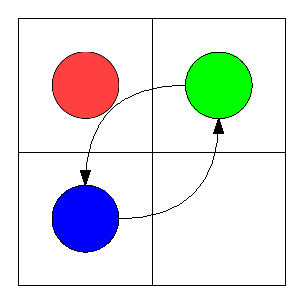
\includegraphics[width=4cm]{include/impossible_2x2.eps}
	\caption{A minimal example of an unsolvable motion planning problem: there exists no valid schedule which swaps the green and blue robots.}\label{fig:reachability}
\end{figure}

% MAKESPAN
\begin{definition}\label{def:makespan}
	The number of single transformation steps in a schedule is called the \emph{makespan} of that schedule.
\end{definition}

\begin{definition}\label{def:optimality}
	Let \(\schedules\) denote the set of all valid schedules for some problem instance \(I\). 
	A schedule \(S_\text{opt}\) is \emph{optimal} with respect to some cost function \(f : \schedules \mapsto \mathbb{N}\) mapping all valid schedules to some integer value if and only if \(f(S) \geq f(\sopt)\) for all such valid schedules \(S \in \schedules\).
\end{definition}

% M3PP -- MINIMUM MAKESPAN MOTION PLANNING PROBLEM
\begin{definition}\label{def:m3pp}
	Let the makespan of a schedule be such a cost function: \(M : S \mapsto \parens{\text{number of steps in S}}\). 
	The \emph{minimum makespan motion planning problem} asks to find an \emph{optimal} schedule with respect to the makespan \(M\) for some input problem instance.
\end{definition}

\begin{remark}
	The \emph{minimum makespan} for any motion planning problem instance \(I \coloneqq \parens{G,\ \conf{s},\ \conf{t}}\) is bounded below by \(\max(\set{\manhattan{\iconf{s}{r}, \; \iconf{t}{r}}, \; r \in R})\).
\end{remark}

\begin{definition}
	Let the aforementioned lower bound to a schedule with makespan \(M\) be denoted by \(L\). 
	The \(\emph{stretch factor}\) for that schedule is then defined as \(\frac{M}{L}\), which is always at least 1. 
\end{definition}

\subsection{Some general notation}

\begin{definition}
	A function \(f(n)\) has an asymptotic upper bound \(g(n)\) if there are some constants \(c \text{ and } n_0\) such that \(f(n) \leq c\cdot g(n),\ \forall n \geq n_0\). 
	It is then denoted as \(f(n) = \mathcal{O}(g(n))\). 
\end{definition}

% Let \emph{A} be some algorithm. 
% \fda{\(A\) is said to run in \emph{polynomial time} ... if the execution of \(A\) by a deterministic Turing machine is done in a polynomial number of steps w.r.t.\ the input bit length... (are yyou sure you want do define this? I think is better to assume it is known)}
% It is \emph{polynomial time} and often said to be \emph{efficient} if the runtime of \emph{A} is bounded by some polynomial function \(T(A) = O(n^c)\) for some constant \(c\).

Let OPT be the optimal (minimum) value of some function \(f\). 
If some algorithm \(A\) can always find a solution that maps to within a \(\rho\)-factor of the optimal value: \(OPT \leq f(x_A) \leq \rho \cdot OPT\), the algorithm is called a \(\rho\)-approximation algorithm. 


% PAPERS 
\section{The general minimum makespan parallel motion planning problem on a grid is NP-hard}\label{chapter:main_proof}

% PRELIMINARIES
\subsection{Theorem-specific preliminaries}

A (deterministic) \emph{Turing Machine} (TM) is a mathematically modeled machine capable of general purpose computations operating on a tape of symbols. 
It is generally considered to be equivalent in capabilities to most mathematical definitions of computation. 
See \cite{aw/HopcroftU79} for a formal definition.

A \emph{decision problem} is a computational problem asking a yes/no question based on some input.

There are different \emph{classes} of decision problems in terms of computational complexity. 
The \emph{P}-class of problems is defined as the set of decision problems solvable by a TM in \emph{polynomial time}, i.e.\ in \(O(n^k)\) time on the size of the input \emph{n} and some constant \emph{k}.

The \emph{NP}-class of problems is defined as the set of decision problems that are \emph{verifiable} by a TM in polynomial time. 
Actually finding a solution to an NP-problem might take considerably longer. 
It remains an important open question whether P is or is not equal to NP, but many believe P is a proper subset of NP.

A transformation of a problem \(B\) into another problem \(A\) such that a solution to \(A\) solves \(B\) is called a \emph{reduction} and is commonly denoted \(B \leq A\). 
If the reduction can be done in polynomial time, we write \(B \leq_p A\).

\begin{definition}\label{def:np_complete}
	A decision problem \emph{A} is \emph{NP-complete} (\(A \in \text{NPC}\)) if and only if \emph{A} is in NP and there exists a polynomial time reduction from every problem in NP to \emph{A}:
	\begin{align*}
		A \in \text{NPC} \Leftrightarrow \parens{A \in \NP} \land \parens{B \leq_p A, \; \forall B \in \NP}
	\end{align*}
	NP-complete is essentially the hardest class of problems that can be verified in polynomial time. 
\end{definition}

\begin{remark}\label{rem:p_np_disjoint}
	If \(\pclass \neq \NP\) holds, the classes of P and NP-complete problems are disjoint. Otherwise \emph{all} problems in NP would be polynomially reducible to problems solvable in polynomial time, thus also solvable themselves in polynomial time. This would imply P = NP:
	\begin{align*}
		& \pclass \cap \text{NPC} \neq \emptyset \\
		\Rightarrow \; & \exists A \in \pclass : B \leq_p A, \; \forall B \in \NP \\
		\Rightarrow \; & B \in \pclass, \; \forall B \in \NP \\
		\Rightarrow \; & \pclass = \NP
	\end{align*}
\end{remark}

\begin{definition}\label{def:np_hard}
	A problem \emph{H} is classified as \emph{NP-hard} if there exists a polynomial time reduction \(A \leq_p H, \; \forall A \in \NP\). 
	Note that \(H\) begin NP-hard does \emph{not} imply \(H \in \NP\). 
	Though if \(H\) can be proven to belong to NP, i.e. be verifiable in polynomial time, \(H\) will then by definition be NP-complete.
\end{definition}

\begin{remark}\label{rem:p_np_hard_disjoint}
	The same construction as in \cref{rem:p_np_disjoint} works here too, P and NP-hard problems are disjoint, assuming \(\pclass \neq \NP\).
\end{remark}

\begin{remark}\label{note:npc_proving}
	Let \(A\) be some known NP-complete problem. 
	If there is a polynomial time reduction from \(A\) to some other problem \(B\): \(A \leq_p B\), we know that \(B\) is NP-hard. 
	Further proving that \(B\) is NP-complete would require \emph{either} a polynomial reduction from \(B\) to \(A\): \(B \leq_p A\) \emph{or}, possibly easier, proving that \(B\) is in NP, i.e. proving that \(B\) is deterministically verifiable in polynomial time.
\end{remark}

Let a \emph{boolean expression} be composed of boolean variables \(b \in \set{\true,\, \false}\), negations (\texttt{not } \(\neg\)), conjunctions (\texttt{and} \(\land\)), disjunctions (\texttt{or} \(\lor\)) and parentheses.

The following is an example of a boolean expression:
\begin{align}\label{ex:boolean_xor}
	\parens{b_1 \lor b_2} \land \neg \parens{b_1 \land b_2}
\end{align}

Let a \emph{literal} be a variable \(b\) (a positive literal) or the negation of a variable \(\neg b\) (a negative literal). 
A (disjunctive) \emph{clause} is then defined as a disjunction of literals \(C = \parens{l_1 \lor l_2 \lor \dots \lor l_k}, \ l_i \in \set{b_j,\ \neg b_j}\). 

Let a boolean expression be in \emph{Conjunctive Normal Form} (CNF) if and only if it is composed only of conjunctions of disjunctive clauses. 
The previous example in \cref{ex:boolean_xor} is \emph{not} in CNF, as negation of a clause is not allowed, and the second parenthesis is a conjunction, not a disjunction.

\begin{remark}
	It is always possible, but non-trivial, to transform an arbitrary boolean expression into CNF \cite{aw/RN2020}.
	The expression in \cref{ex:boolean_xor} can be stated in CNF as follows:
	\begin{align}\label{ex:cnf_xor}
		\parens{b_1 \lor b_2} \land \parens{\neg b_1 \lor \neg b_2}
	\end{align}
\end{remark}

Let \(\varphi\) be a boolean expression in Conjunctive Normal Form. 
The boolean satisfiability problem, abbreviated \emph{SAT}, is a decision problems asking whether \(\varphi\) can be evaluated to \true\ for some state of its variables \(\set{b_1, b_2, \dots, b_n} \in \set{\true, \false}^{n}\). 
It is trivial to verify if a solution is correct or not: a boolean expression can be evaluated well within polynomial time, thus SAT has to be in NP. 
On the other hand, there are an exponential amount of states of the input variables: \(2^n\) states for the \(n\) input variables to be exact. 
It has been proven that SAT is NP-complete \cite{coco/Karp72}, and a sub-exponential algorithm for solving a general SAT problem would be groundbreaking. 

The corresponding SAT problem to \cref{ex:cnf_xor} would ask whether \(\varphi\) is satisfiable. 
This particular expression is satisfiable, as when \(\coord{b_1}{b_2} = (\true, \false)\) or \(\coord{b_1}{b_2} = \coord{\false}{\true}\) the expression evaluates to \true, coincidentally equivalent to an \texttt{xor}\ expression.

\begin{definition}
	\emph{3SAT} is a sub-problem of SAT where each input instance has exactly 3 literals in each clause. 
	3SAT is also known to be NP-complete.
\end{definition}

\begin{definition}
	A \emph{Monotone 3SAT} is defined as a further restricted version of 3SAT, where each clause of the expression has all-positive or all-negative literals.
\end{definition}

% Boolean expressions are constructed from positive and negative literals (\(x} and \(\neg x} respectively), conjunctions (AND \(\land}), disjunctions (OR \(\lor}) and parentheses. An example SAT problem would ask whether \(}









% MAIN THEOREM
\subsection{The theorem}

Let a decision problem formulation of minimum makespan motion planning be as follows: Given a problem instance \(I \coloneqq \parens{G,\ \conf{s},\ \conf{t}}\), determine if there exists a schedule with makespan at most \emph{M} that can transform \(\conf{s} \rightarrow \conf{t}\).

\begin{lemma}\label{lemma:np}
	The decision problem formulation of a minimum makespan motion planning problem on a grid is in NP.
\end{lemma}

\begin{proof}
	It is easy to show that the decision problem is in NP; to verify a found solution, one has to check three things:
	\begin{enumerate}
		\item Every transformation step of a schedule should be valid according to \cref{req:limited_movement} and \cref{req:no_swaps}.\label{checks:transformations}
		\item After the last step of execution, the configuration should equal that of \(\conf{t}\).\label{checks:target_acquired}
		\item There should be at most \(M\) transformation steps.\label{checks:makespan}
	\end{enumerate}
	\cref{req:limited_movement} can be checked in linear time with respect to the robots for each timestep. 
	\cref{req:no_swaps} will need to be checked for each single-robot move, which is bounded by the number of robots for each timestep. 
	Thus \cref{checks:transformations} can be checked in \(\mathcal{O}(M \cdot N)\) time, where \(M\) is the makespan and \(N\) is the number of robots.
	\cref{checks:target_acquired} can be done linearly with respect to the number of robots, as checking the positions for every robot is sufficient (configurations are assumed to be valid, and that \(\iconf{}{r}\) would raise an error if the mapped position would not be deterministically defined).
	Trivially \cref{checks:makespan} can be done in \(\mathcal{O}(M)\). 
	% \fda{be careful, because items 1 and 2 need also to be repeated for at most \(M\) times: it needs to be added in the final running time}
	% ^^ should be accounted for already

	A solution is thus verifiable in \(\mathcal{O}(M \cdot N)\), which implies the problem is in NP by definition.
\end{proof}

\begin{theorem}\label{thm:npc}
	The decision problem formulation of a minimum makespan motion planning problem on a grid is NP-complete.
\end{theorem}

\begin{proof}
	The following proof, heavily based on the proof by \cite{siamcomp/DemaineFKMS19} is done by a polynomial reduction from \emph{Monotone 3SAT} to a decision formulation of a coordinated multi-robot motion planning problem. 
	As Monotone 3SAT is known to be NP-complete, a polynomial reduction implies the reduced problem is NP-hard. 
	Together with \cref{lemma:np}, this implies the problem is also NP-complete. 






% REDUCTION
	\subsubsection*{The reduction} 
	Let \(\varphi\) be some boolean expression corresponding to some Monotone 3SAT problem. 
	The idea is to construct a workspace with robots having start and target configurations \(\conf{s}\) and \(\conf{t}\) respectively such that a critical makespan \emph{M} is achievable if and only if the original expression \(\varphi\) is satisfiable, otherwise requiring \(M + 1\) transformation steps at a minimum to transform \(\conf{s} \rightarrow \conf{t}\). 
	Follow along the construction by observing \cref{fig:full_reduction}: a one-to-one sketch of the simplest possible example. 





% FIGURE
\begin{figure}[h]
	\centering
	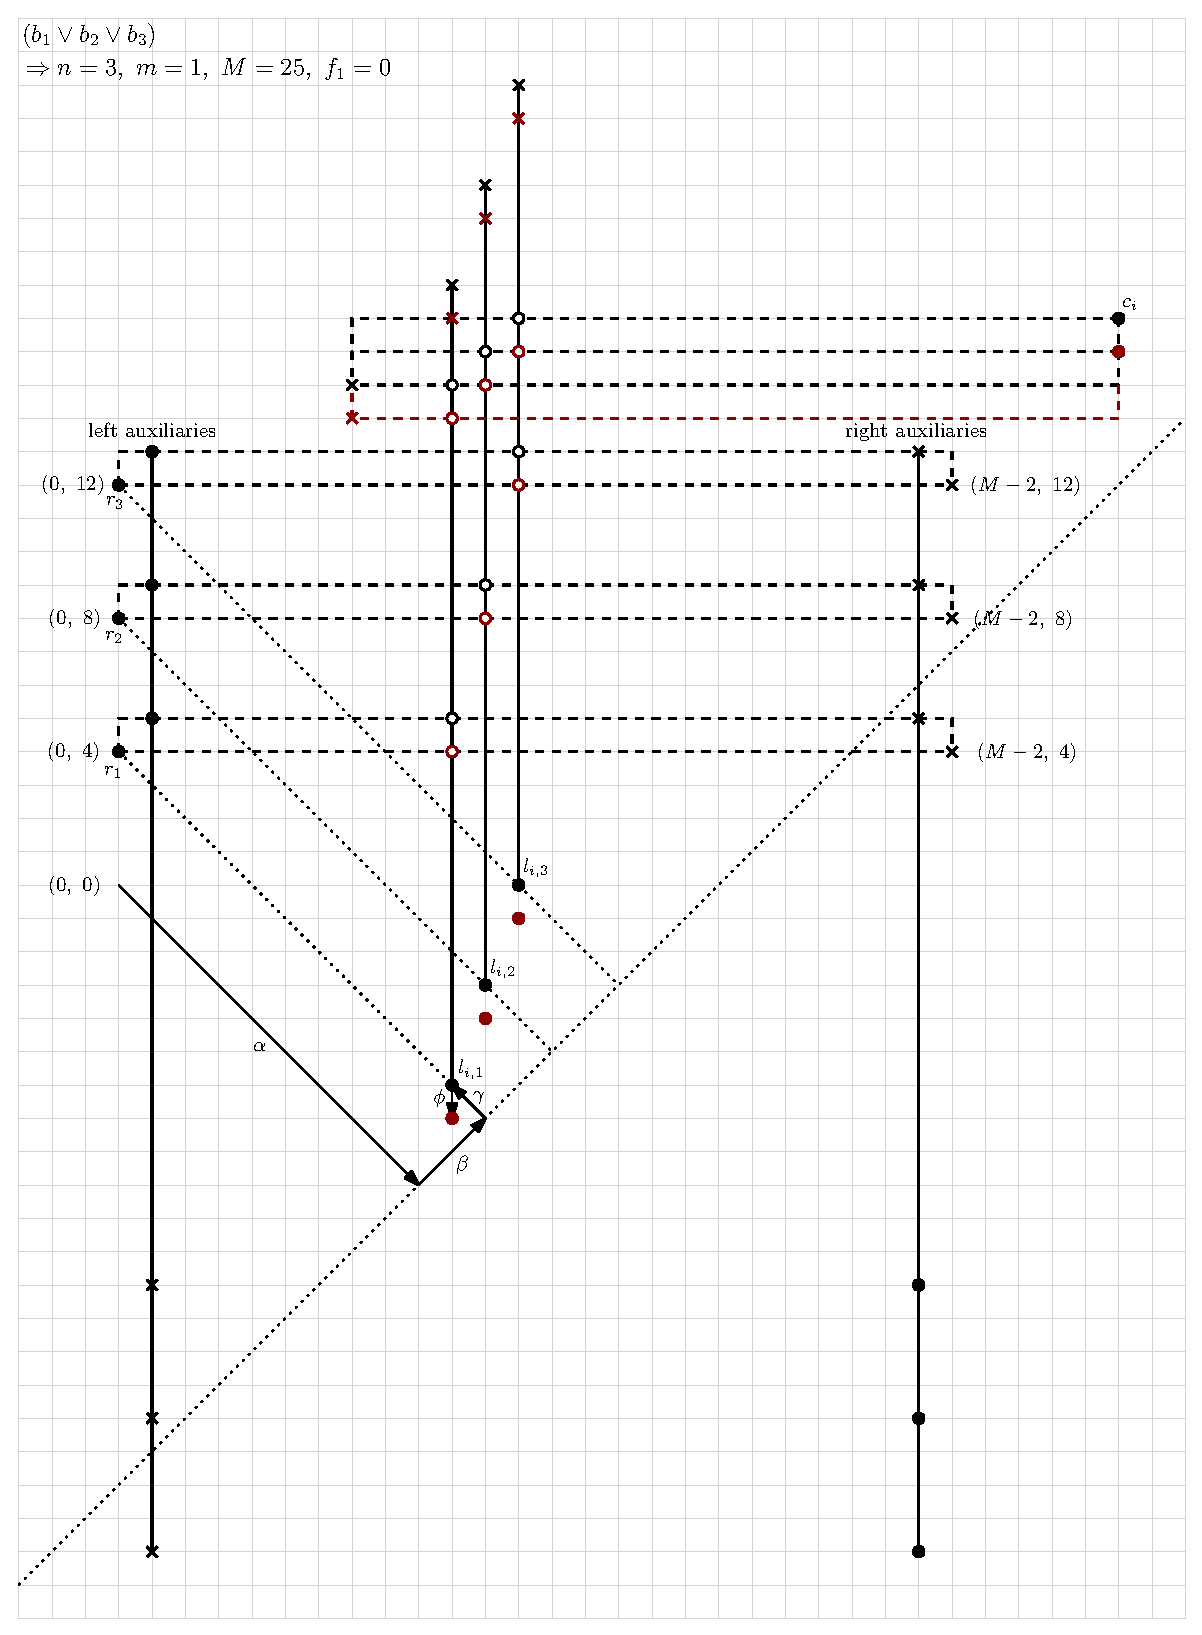
\includegraphics[height=15cm]{ipe/np_reduction.eps}
	\caption{
		A minimal Monotone 3CNF formula \(\varphi = \parens{b_1 \lor b_2 \lor b_3}\) reduced to a robot motion planning problem. 
		The dark red graphics show how the robots would be offset if the clause \(c_i\) was all-negative instead of the current all-positive. 
		Disks represent robots while crosses represent their target positions. 
		The circles highlight the variable-literal couplings and literal-clause couplings: a mismatched assignment of \(b_{j_k}\) w.r.t. \(l_{i,k}\) cascades into \(l_{i,k}\) blocking the path of \(c_i\).
	}\label{fig:full_reduction}
\end{figure}





	% Let our target makespan \emph{M} be fixed at the end of the construction, so that a schedule with makespan \emph{M} is achievable if and only if the original expression \(\varphi\) is satisfiable, otherwise a schedule with makespan \(M + 1\). 

	The formula \(\varphi\) is composed of \(n\) boolean variables \(\set{b_1, b_2, \dots, b_n}\) and \(m\) clauses \(\set{C_1, C_2, \dots, C_m}\) with three literals each. 
	Let our variables be represented by \(n\) \emph{variable robots} \(\set{r_1, r_2, \dots, r_n}\). 
	These will be able to `choose' one of two paths independently of one another, representing \true\ and \false\ assignments to them. 
	The variable robots are coupled in a many-to-many mapping to the clauses by \(3m\) \emph{literal robots}: \(\set{l_{i,k} \mid i \in \set{1, \dots, m},\ k \in \set{1, 2, 3}}\). 
	They are positioned so that they pass by their corresponding variable robot, and have to wait if the variable assignment is mismatched with the literal. 
	There are finally \(m\) \emph{clause robots} to ensure that at least one literal per simulated clause evaluates to \true. 
	This is accomplished by the clause robot having a clear path to its target only if at least one corresponding literal robot has not needed to wait for its variable robot. 
	The workspace is constructed so that any robot deviating from its constrained path results in a schedule with makespan \(> M\).

	% is made so a makespan \(M\) is only achievable if every clause robot is not blocked by a literal robot on its path, and all robots are constrained by the makespan to behave like .

	There are some details to deal with: the variable robots have to be constrained to be able to take exactly two distinct paths, while the literal robots have to be positioned to get the correct timing with its corresponding variable robot and clause robot simultaneously.

	Let the variable robot \(r_j\) have a start position at \(\coord{0}{4j}\) and target position at \(\coord{M - 2}{4j}\). 
	Notice there is exactly two timesteps to spare with respect to the critical makespan \(M\). 
	Let there be a \emph{left auxiliary robot} and a \emph{right auxiliary robot} for each variable robot. 
	The left auxiliary starts at \(\coord{1}{4j + 1}\) and travels down to \(\coord{1}{4j + 1 - M}\), while the right auxiliary starts at \(\coord{M - 3}{4j + 1 - M}\), and moves up to \(\coord{M - 3}{4j + 1}\). 
	The auxiliaries have to move exactly \(M\) steps, and thus cannot wait for \(r_j\). 
	Thus \(r_j\) is blocked from moving right at timestep 0 by the left auxiliary, and required to pass \(x = M - 3\) before timestep \(M\) to avoid blocking the right auxiliary. 
	As a result, \(r_j\) has exactly two options: wait at timesteps \(0\) and \(M\), alternatively move up at timestep \(0\) and down at timestep \(M\). 
	This constrains \(r_j\) to move monotonously to the right between steps 1 and \(M - 1\).

	% Let the clause robot \(c_i\) have start and target positions such that it has to move exactly \(M-2\) steps left and \(2\) steps down. We will construct the paths of our literal robots such that they block the \emph{upper, middle} and \emph{lower} vertical levels in sequence: if the clause robot is blocked first at the uppermost level, it has no choice but move one level down and continue. If it is again blocked at the middle level, it has to move down a last time. At the lowest level, a blockage forces the clause robot to wait. % We will construct the paths of the literal robots to block the clause robot precisely like this. 

	Let the literal robots \(\set{l_{i,1}, l_{i,2}, l_{i,3}}\) of clause \(C_i\) correspond to the variable robots \(\set{r_{j_1}, r_{j_2}, r_{j_3}},\ j_1 < j_2 < j_3\). 
	Let \(f_i = -1\) if \(C_i\) is negative, \(f_i = 0\) otherwise. 
	Finally, define the vectors \(\set{\alpha,\ \beta,\ \gamma,\ \phi}\):
	\begin{align*}
	\alpha \coloneqq \colvec{3n}{-3n} \quad 
	\beta \coloneqq \colvec{2}{2} \quad 
	\gamma \coloneqq \colvec{-1}{1} \quad 
	\phi \coloneqq \colvec{0}{1}
	\end{align*}

	Set the starting position of literal robot \(l_{i,k}\) to be \(\parens{\alpha \cdot i + \beta \cdot j_k + \gamma \cdot k + \phi \cdot f_i}\). 
	The target position of \(l_{i,k}\) is simply \(M - 1\) steps above its start position. 
	Note the literal robots can wait for up to one timestep.


	Denote the target position of \(l_{i,1}\) as \(t_{i,1} \parens{= \alpha \cdot i + \beta \cdot j_1 + \gamma + \phi \cdot f_i}\) for a moment. 
	Set the start and target positions of the clause robot \(c_i\) to \(t_{i,1} + \coord{M - 5}{-1}\) and \(t_{i,1} - \coord{3}{3}\) respectively. 
	Note that the clause robot has to move \(M - 2\) steps to the left and \(2\) steps down and cannot wait, so it requires a clear path towards its target to make it within makespan \(M\).
	
	Note the importance of the two diagonals for robot-robot timings here: they are reminiscent of the eigenvectors of a matrix. 
	Repositioning the literal robot along the downwards \diagdegs diagonal, the timing with respect to the variable robots, which move to the right, does not change, only the horizontal intersection of their paths, i.e. the two robots will still collide just the same. 
	Similarly, repositioning the literal robot along the upwards diagonal does not change its timing with respect to a clause robot, which start at the top and move left. 

	Now, onto explaining the specificity of the literal robot positioning. 
	As hinted above, the position of the literal robots \(\set{l_{i,1},\ l_{i,2},\ l_{i,3}}\) are each individually close to the downwards diagonal starting at their corresponding variable robot \(r_{j_k}\), which the offset \(\beta \cdot j_k\) takes care of. 
	Among themselves, they are also close to the same upwards diagonal, which times them correctly with respect to their clause robot. 
	The offset \(\alpha \cdot i\) puts them at the same diagonal, separating them from the literals of the clauses \(c_{i-1} \text{ and } c_{i+1}\). 
	Finally, \(\gamma \cdot k\) staggers the three literals such that \(l_{i,3}\) is one step ahead of \(l_{i,2}\), which is one step ahead of \(l_{i,1}\) (w.r.t the clause robot \(c_i\)). 
	This, combined with the specific positioning of \(c_i\), makes it so \(c_i\) has three functionally distinct paths, which are individually blocked by its three literals when their respective variables are mismatched.

	The purely vertical negative offset \(\phi\) when \(C_i\) is all-negative results in \(l_{i,k}\) going from `colliding' with a \false\ \(r_{j_k}\) to `colliding' when \(r_{j_k} = \true\). 
	All literal robots \(l_{i,k}\) and the clause robot \(c_i\) that correspond to clause \(C_i\) get this same offset, so their relative timings are unaffected.
	
	The only thing left is determining the critical makespan \(M\): all literal robots have to fit in between the left and right auxiliary-robots, while all variable robots should fit in the span of all the literal robots, with some room to spare for the lowest clause robot \(c_m\).

	\begin{align*}
		& M = \max \parens{
			\underbrace{3nm + 2n + 1}_{
				\substack{
					\text{Horizontal} \\
					\text{space for \(l_{m,3}\)} \\
					\text{ and auxiliaries}
				}
			}, \quad
			\underbrace{3nm + 4n + 4}_{
				\substack{
					\text{Vertical space} \\
					\text{for \(r_n\) and \(c_m\)} \\
					\text{within span of \(l_{i,1}\)}
				}
			}
		} \\
		\Rightarrow & M = 3nm + 4n + 4 \ \text{is sufficient}
	\end{align*}

	As a result of this construction, an arbitrary Monotone 3SAT problem can be simulated with coordinated robots on a grid. 
	A makespan of \(M = 3nm + 4n + 4\) is achievable if and only if every clause robot has a clear path, implying they all have at least one satisfied literal. 
	This implies \(\varphi\) is satisfiable if and only if there is a schedule with makespan \(M\) that transforms the workspace from \(\conf{s} \rightarrow \conf{t}\).
\end{proof}


Compared to the construction in the original proof by \cite{siamcomp/DemaineFKMS19}, this construction works with a smaller makespan: \(3nm + 4n + 4\) versus \(6n(m + 2)\) for the proof in \cite{siamcomp/DemaineFKMS19}. 
The number of needed robots is also significantly smaller: \(3n + 4m\) robots compared to \(3n + 3m + 6n(m + 2)\) robots in the original. 

\begin{corollary}
	The problem of computing a \emph{minimum} makespan schedule for a given problem instance is as hard as the corresponding decision problem. 
\end{corollary}

\begin{proof}
	Assume that there exists an efficient solution to the minimum makespan problem: it would trivially solve the decision problem efficiently. This implies the minimum makespan problem has to be at least as hard as the decision problem. 

	
	Assume instead there exists an algorithm \(A\) that solves the decision problem. 
	It has runtime \(T(A)\). 
	\cite{siamcomp/DemaineFKMS19} shows that the optimal makespan is bounded above by \(\mathcal{O}(n_1 + n_2)\). 
	Thus, repeatedly applying \(A\) for makespans \(\set{1, 2, \dots, \mathcal{O}(n_1 + n_2)}\) would solve the minimum makespan problem within \(\mathcal{O}(T(A) \cdot (n_1 + n_2) )\) time. 
	This is exponential if \(T(A)\) is exponential, polynomial if \(T(A)\) is polynomial. 
	Thus the minimum makespan problem is not harder than the decision problem. 

	This proves the minimum makespan problem has to be as hard as the corresponding decision problem.
\end{proof} 

Classifying the complexity of parallel robot motion planning as NP-complete is important, as it shows that it is unfeasible to compute an optimal schedule for sufficiently large problem instances. 
This implies that real world use requires efficient approximation algorithms.



\section{Reconfiguration by swap operations}

\subsection{Specific preliminaries}

\subsubsection{Definitions}

\subsection{Swapping two neighboring robots is a constant time operation}

\cite{siamcomp/DemaineFKMS19} 

\section{Alternative metrics to makespan}\label{chapter:alternative_metrics}

Let \(\alpha_r \coloneqq \max\set{\tau' \mid \iconf{\tau}{r} = \iconf{t}{r}\ \forall \tau \geq \tau'}\) be the arrival time of \(r\), i.e. the timestep when \(r\) stops moving. 
Define \(P_r \coloneqq \set{ \parens{ \iconf{i}{r},\ \iconf{i + 1}{r} } \mid \parens{ \iconf{i}{r},\ \iconf{i + 1}{r} } \in E }\) to be the \emph{path} of \(r\): the sequence of steps \(r\) takes in a schedule. 

Then consider the following well-defined cost functions:
\begin{align*}
	% \smash and manual spacing to circumvent the larger block from \max_{r \in R}
	& \mono{Makespan} 				& \mono{(M)} && \schedules \mapsto \quad & \smash{\max_{r \in R}} \ \alpha_r 	\\[2mm] 
	& \mono{Total Arrival Time} 	& \mono{(TAT)} && \schedules \mapsto \quad & \Sigma_{r \in R} \ \alpha_r 		\\[2mm]
	& \mono{Total Distance} 		& \mono{(TD)} && \schedules \mapsto \quad & \Sigma_{r \in R} \ \abs{P_r} 		\\[2mm]
	& \mono{Maximum Distance} 		& \mono{(MD)} && \schedules \mapsto \quad & \max_{r \in R} \ \abs{P_r}
\end{align*}

% \cite{corr/YuL15c} examines all four of these on a general graph, i.e. not contrained to model a grid like in our case. An important finding is proving the decision problem statements for the respective optimization problems of the cost functions above are all NP-complete on a general graph. This importantly does \emph{not} imply the same holds for the grid case of coordinated robot motion planning, and the reduction they use is not easily convertible to the grid. It seems currently unknown if the respective decision problems to these metrics are also NP-complete on the grid similar to \cref{thm:npc}.

\cite{corr/YuL15c} finds that for a robot motion planning problem on a \emph{general} graph, one cannot always find schedules that optimize any pair of the above cost functions simultaneously: 
\begin{align}\label{eq:metric_tuple}
	\forall \parens{f_1,\ f_2} \in \set{\mono{M, TAT, TD, MD}}^2 : \exists I : \schedules_{\text{opt}_{f_1}} \cap \schedules_{\text{opt}_{f_2}} = \emptyset,
\end{align}
where \(\schedules_{\text{opt}_f} \subseteq \schedules\) denotes the set of optimal schedules for an instance \(I\) with respect to some cost function \(f\). 
That \cref{eq:metric_tuple} is true on a general graph does not imply that it holds for our problem formulation on a grid, and the graphs used in the proof are not compatible with our grid-model. 
However, by coming up with new grid-specific problem instances we prove the statement holds on the grid as well.

\begin{lemma}\label{lemma:simultaneous_1}
	A pairing of cost functions \(\parens{f_1, f_2} \in \set{\mono{M, MD}} \times \set{\mono{TAT, TD}}\) cannot always be simultaneously optimized on the grid.
\end{lemma}

\begin{proof}
	% FIGURE SIMULTANEOUS 1 PROBLEM
	\begin{figure}[h]
		\centering
		
\includegraphics[width=0.35\linewidth]{ipe/sim1_problem.eps}
		\caption{
			A problem instance that requires different schedules depending on the cost function. Circles represent robots, crosses represent their targets. The two robots in the middle are already on their targets. 
		}
		\label{fig:sim1}
	\end{figure}

	Observe the configuration in \cref{fig:sim1}. 
	It is easy to see that there are two different ways to schedule a solution: either sacrifice maximum time and distance by letting the single robot move around the two central ones, or alternatively let the middle robots move out of the way, sacrificing the total travel time and distance instead. 
	See \cref{fig:sim1_strat} for a visual of this. 

	% FIGURE SIMULTANEOUS 1 STRATEGIES
	\begin{figure}[h]
		\centering
		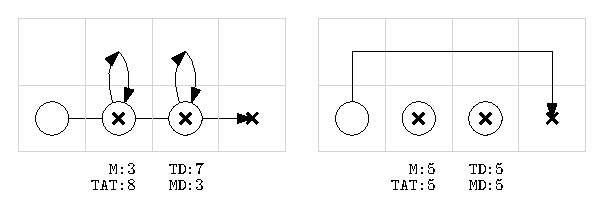
\includegraphics[width=0.7\linewidth]{ipe/sim1_strat.eps}
		\caption{
			The left schedule optimizes \mono{M}\ and \mono{MD}, while the right schedule optimizes \mono{TD}\ and \mono{TAT}.
		}
		\label{fig:sim1_strat}
	\end{figure}

It is quite trivial to conclude that there are no better solutions to this instance w.r.t. these metrics. 
This implies one cannot always optimize simultaneously for any pairing in \(\set{\mono{M, MD}} \times \set{\mono{TAT, TD}}\) on the grid.
\end{proof}

\begin{lemma}\label{lemma:simultaneous_2}
	A pairing of cost functions \(\parens{f_1, f_2} \in \set{\mono{M, TAT}} \times \set{\mono{MD, TD}}\) cannot always be simultaneously optimized for on the grid. 
\end{lemma}

\begin{proof}
	% FIGURE SIMULTANEOUS 2 PROBLEM
	\begin{figure}[h]
		\centering
		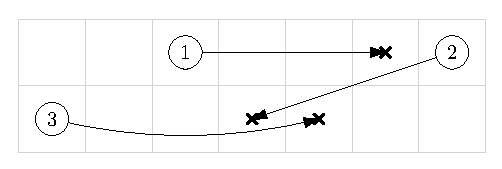
\includegraphics[width=0.45\linewidth]{ipe/sim2_problem.eps}
		\caption{
			A second instance that requires different schedules depending on the cost function.
		}
		\label{fig:sim2}
	\end{figure}

	% FIGURE SIMULTANEOUS 2 STRATEGIES
	\begin{figure}[h]
		\centering
		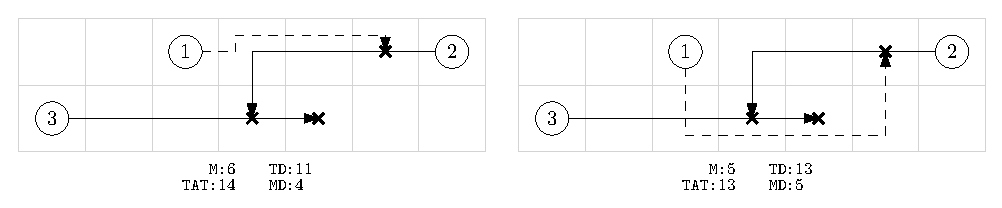
\includegraphics[width=\linewidth]{ipe/sim2_strat.eps}
		\caption{
			The left schedule optimizes \mono{TD}\ and \mono{MD}, while the right schedule optimizes \mono{M}\ and \mono{TAT}.
		}
		\label{fig:sim2_strat}
	\end{figure}

	Similarly to \cref{lemma:simultaneous_1}, observe the instance in \cref{fig:sim2}. 
	There are again two different strategies, seen in \cref{fig:sim2_strat}: robot 1 either waits for robot 2 to pass, or alternatively goes a longer distance beneath robot 2. 
	The instance is constructed so 2 and 3 have no choice but to move in these specific paths to avoid accumulating larger time and distance penalties, which means 1 has the only real choice here. 
	As there are no better schedules than these for any of these metrics, it implies no schedule exists that optimizes the specific pairs in \cref{lemma:simultaneous_2} concurrently.
\end{proof}

\begin{theorem}
	A pair of cost functions \(\parens{f_1, f_2} \in \set{\mono{M, TAT, TD, MD}}^2 \) cannot always be simultaneously optimized for on the grid. 
\end{theorem}

\begin{proof}
	\begin{figure}[h]
		\centering
		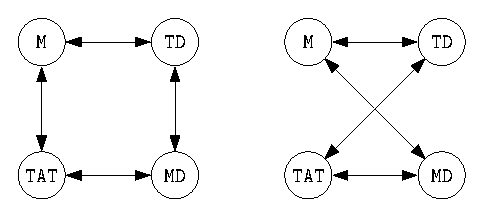
\includegraphics[width=0.5\textwidth]{ipe/sim_thm.eps}
		\caption{
			The pairs of sometimes simultaneously unoptimizable cost functions given \cref{lemma:simultaneous_1} and \cref{lemma:simultaneous_2} respectively.
		}
		\label{fig:sim_separate}
	\end{figure}

	Consider the graphs in \cref{fig:sim_separate} that show which cost functions are sometimes pairwise simultaneously unoptimizable. 
	A new graph with the same vertices and a union of the edges clearly gives us a 4-clique, which is exactly what we are after. 
	This implies the general proof from \cite{corr/YuL15c} also holds on the grid.
\end{proof}



% CONCLUSIONS

\section{Conclusions}
% \fda{develop section as discussed in the meeting}

We have looked at several important aspects of coordinated multi-robot motion planning on the grid:

In \cref{chapter:main_proof} we proved that the decision problem of minimum makespan motion planning is NP-complete using a simplified version of a reduction from \cite{siamcomp/DemaineFKMS19}. 
The proof uses substantially fewer robots than the original, which should make it easier to grasp. 
The proof is important in that it shows the value of efficient approximation algorithms in the field of parallel robotics. 

In \cref{chapter:constant_stretch} we took a high-level look at some of the approximation algorithms introduced by \cite{siamcomp/DemaineFKMS19}, which can efficiently compute schedules with constant stretch, implying a guaranteed level of robot performance even in large problem instances.

Lastly, in \cref{chapter:alternative_metrics} we extended a theorem from \cite{corr/YuL15c} from holding on general graphs to also hold specifically on the grid: considering four distinct cost functions, any pairing cannot always be simultaneously optimized.
The theorem shows the importance of choosing the right cost function when optimizing solutions to motion planning problems. 

Only a small part of the field of coordinated motion planning was covered though. 
Still left untouched are various different problem formulations, especially motion planning modeled in the continuous space seems central for future research.


%% REFERENCES
% \bibliographystyle{aaltosci_t}
\bibliographystyle{ieeetr}
\bibliography{manual_refs}
% \bibliography{manual_refs}
% \printbibliography

\clearpage

%% ADD POSSIBLE APPENDIX HERE
\thesisappendix

\end{document}
